\documentclass[conference,10pt,letterpaper]{IEEEtran}
\usepackage[T1]{fontenc}
\usepackage{amsmath,booktabs,graphicx,url,tikz,float,multirow}
\usetikzlibrary{arrows.meta,positioning}
\definecolor{csiBlue}{RGB}{34,105,158}
\definecolor{radarOrange}{RGB}{198,93,34}
\definecolor{fusionRed}{RGB}{156,40,67}
\renewcommand{\topfraction}{.95}
\renewcommand{\dbltopfraction}{.95}
\renewcommand{\textfraction}{.04}
\renewcommand{\floatpagefraction}{.85}
\renewcommand{\dblfloatpagefraction}{.85}
\setcounter{topnumber}{4}
\setcounter{dbltopnumber}{4}
\graphicspath{{icc_assets/}}
\title{Explainable and private LLM-based Occupancy Detection Model Framework with Multi-Modal Wireless Sensing:\\WiFi CSI and FMCW Radar}
\author{\IEEEauthorblockN{Gad Gad\IEEEauthorrefmark{1}, Mostafa Fouda\IEEEauthorrefmark{2}, Zubair Md Fadlullah\IEEEauthorrefmark{1}}
\IEEEauthorblockA{\IEEEauthorrefmark{1}Department of Computer Science, Western University, London, ON, Canada\\
\IEEEauthorrefmark{2}Department of Electrical and Computer Engineering, Idaho State University, Pocatello, ID, USA}}
\begin{document}
\maketitle
\begin{abstract}

Human occupancy detection using wireless sensing provides private continuous monitoring, but signal instability and distribution shift challenge model performance. Machine-learning predictions also offer limited explanations. We combine WiFi channel-state information (CSI) and frequency-modulated continuous-wave (FMCW) radar to predict room occupancy. Physical descriptors and trained-model probabilities are supplied to large language models (LLMs) for a prediction and textual rationale. We evaluate CSI, radar, early feature fusion, and late probability fusion on fifteen-second windows and minute averages; validation data select models and thresholds before multilink test evaluation. The window models combine the physical descriptors with mean/std summaries of a three-level hierarchical PCA (one-second, five-second, and fifteen-second levels, two components each) whose every level is fitted on the training output of the level below. Among the validation-selected models, the CSI RF achieves .846/.687 validation/test minute accuracy, the radar RF .593/.969, the early-fusion GBM .812/.808, and the late-fusion RF .837/.975. GPT-4o mini scores $58.6\pm2.3$\% validation and $61.1\pm2.2$\% test accuracy, while GPT-5.4 scores $80.4\pm1.5$\% and $94.4\pm0.2$\%, respectively. Late probability fusion machine learning model is the best performing model, and GPT-5.4 approaches its performance while providing explainability.

\end{abstract}
\begin{IEEEkeywords}
occupancy sensing, WiFi CSI, FMCW radar, domain shift, calibration
\end{IEEEkeywords}

\section{Introduction}\label{sec:intro}
Room occupancy is a basic input for lighting, heating, and ventilation control, security, and in-home care. Camera-based occupancy detection raises privacy concerns, and wearable or infrared alternatives require cooperation or line of sight. Radio-frequency sensing offers a passive alternative: WiFi channel-state information (CSI) from commodity transceivers reflects multipath changes caused by a human body, and millimeter-wave frequency-modulated continuous-wave (FMCW) radar supplies range, angle, and Doppler maps that respond to body motion and micro-motion.

Both modalities, however, are sensitive to the acquisition geometry. Moving a receiver to a different wall changes the dominant multipath components, the radar field of view, and the amplitude statistics on which a trained classifier depends. A model that separates the two classes almost perfectly on data from the training placement can therefore fail on data from a new placement, and this failure is often invisible when the validation set shares the training geometry. Machine-learning predictions also arrive without a rationale, which limits their use by operators who must decide whether to trust an alert.

This paper studies these two problems on a single-subject, single-room dataset in which the training placements and the evaluation placement differ by design (Fig.~\ref{fig:layout}). The main contribution of this paper is a multimodal occupancy pipeline that extracts physical descriptors and three-level hierarchical training-basis PCA descriptors from CSI amplitude and from logged radar range--Doppler (RD), range--angle (RA), range--elevation (RE), and Cartesian (XY) maps, and compares CSI-only, radar-only, early feature fusion, and late probability fusion across four model families and five seeds under one frozen protocol: augmented balanced development sets, validation-selected models and thresholds, and a held-out test placement that updates no component.

The remainder of the paper presents related work (Section~\ref{sec:related}), the problem definition (Section~\ref{sec:problem}), the system model (Section~\ref{sec:system}), the collection and processing protocol (Section~\ref{sec:data}), the predictive models (Section~\ref{sec:models}), the language-model inference (Section~\ref{sec:llm}), the results (Section~\ref{sec:results}), the limitations (Section~\ref{sec:limits}), and the conclusion (Section~\ref{sec:conclusion}).

\begin{figure}[!b]
\centering
\resizebox{\columnwidth}{!}{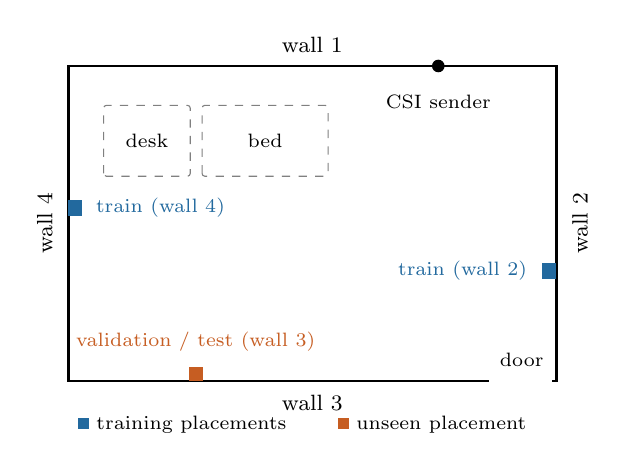
\begin{tikzpicture}[font=\footnotesize]
\draw[line width=1pt] (0,0) rectangle (6.2,4);
\draw[white,line width=1.6pt] (5.35,0) -- (6.15,0);
\draw[line width=1pt] (0,0) -- (5.35,0) (6.15,0) -- (6.2,0);
\node[font=\scriptsize] at (5.76,.27) {door};
\node[anchor=south] at (3.1,4.05) {wall 1};
\node[anchor=north] at (3.1,-.05) {wall 3};
\node[rotate=90] at (-.3,2) {wall 4};
\node[rotate=90] at (6.5,2) {wall 2};
\draw[gray,dashed,rounded corners=1pt] (.45,2.6) rectangle (1.55,3.5);
\node[font=\scriptsize] at (1,3.05) {desk};
\draw[gray,dashed,rounded corners=1pt] (1.7,2.6) rectangle (3.3,3.5);
\node[font=\scriptsize] at (2.5,3.05) {bed};
\fill (4.7,4) circle (.08);
\node[font=\scriptsize,anchor=north] at (4.7,3.75) {CSI sender};
\fill[csiBlue] (0,2.1) rectangle (.18,2.3);
\node[font=\scriptsize,text=csiBlue,anchor=west] at (.23,2.2) {train (wall 4)};
\fill[csiBlue] (6.02,1.3) rectangle (6.2,1.5);
\node[font=\scriptsize,text=csiBlue,anchor=east] at (5.95,1.4) {train (wall 2)};
\fill[radarOrange] (1.53,0) rectangle (1.71,.18);
\node[font=\scriptsize,text=radarOrange,anchor=south] at (1.62,.25) {validation / test (wall 3)};
\node[font=\scriptsize,anchor=west] at (0,-.55) {\textcolor{csiBlue}{\rule{.14cm}{.14cm}} training placements};
\node[font=\scriptsize,anchor=west] at (3.3,-.55) {\textcolor{radarOrange}{\rule{.14cm}{.14cm}} unseen placement};
\end{tikzpicture}}
\par\smallskip
\begin{minipage}[c]{.49\columnwidth}\centering
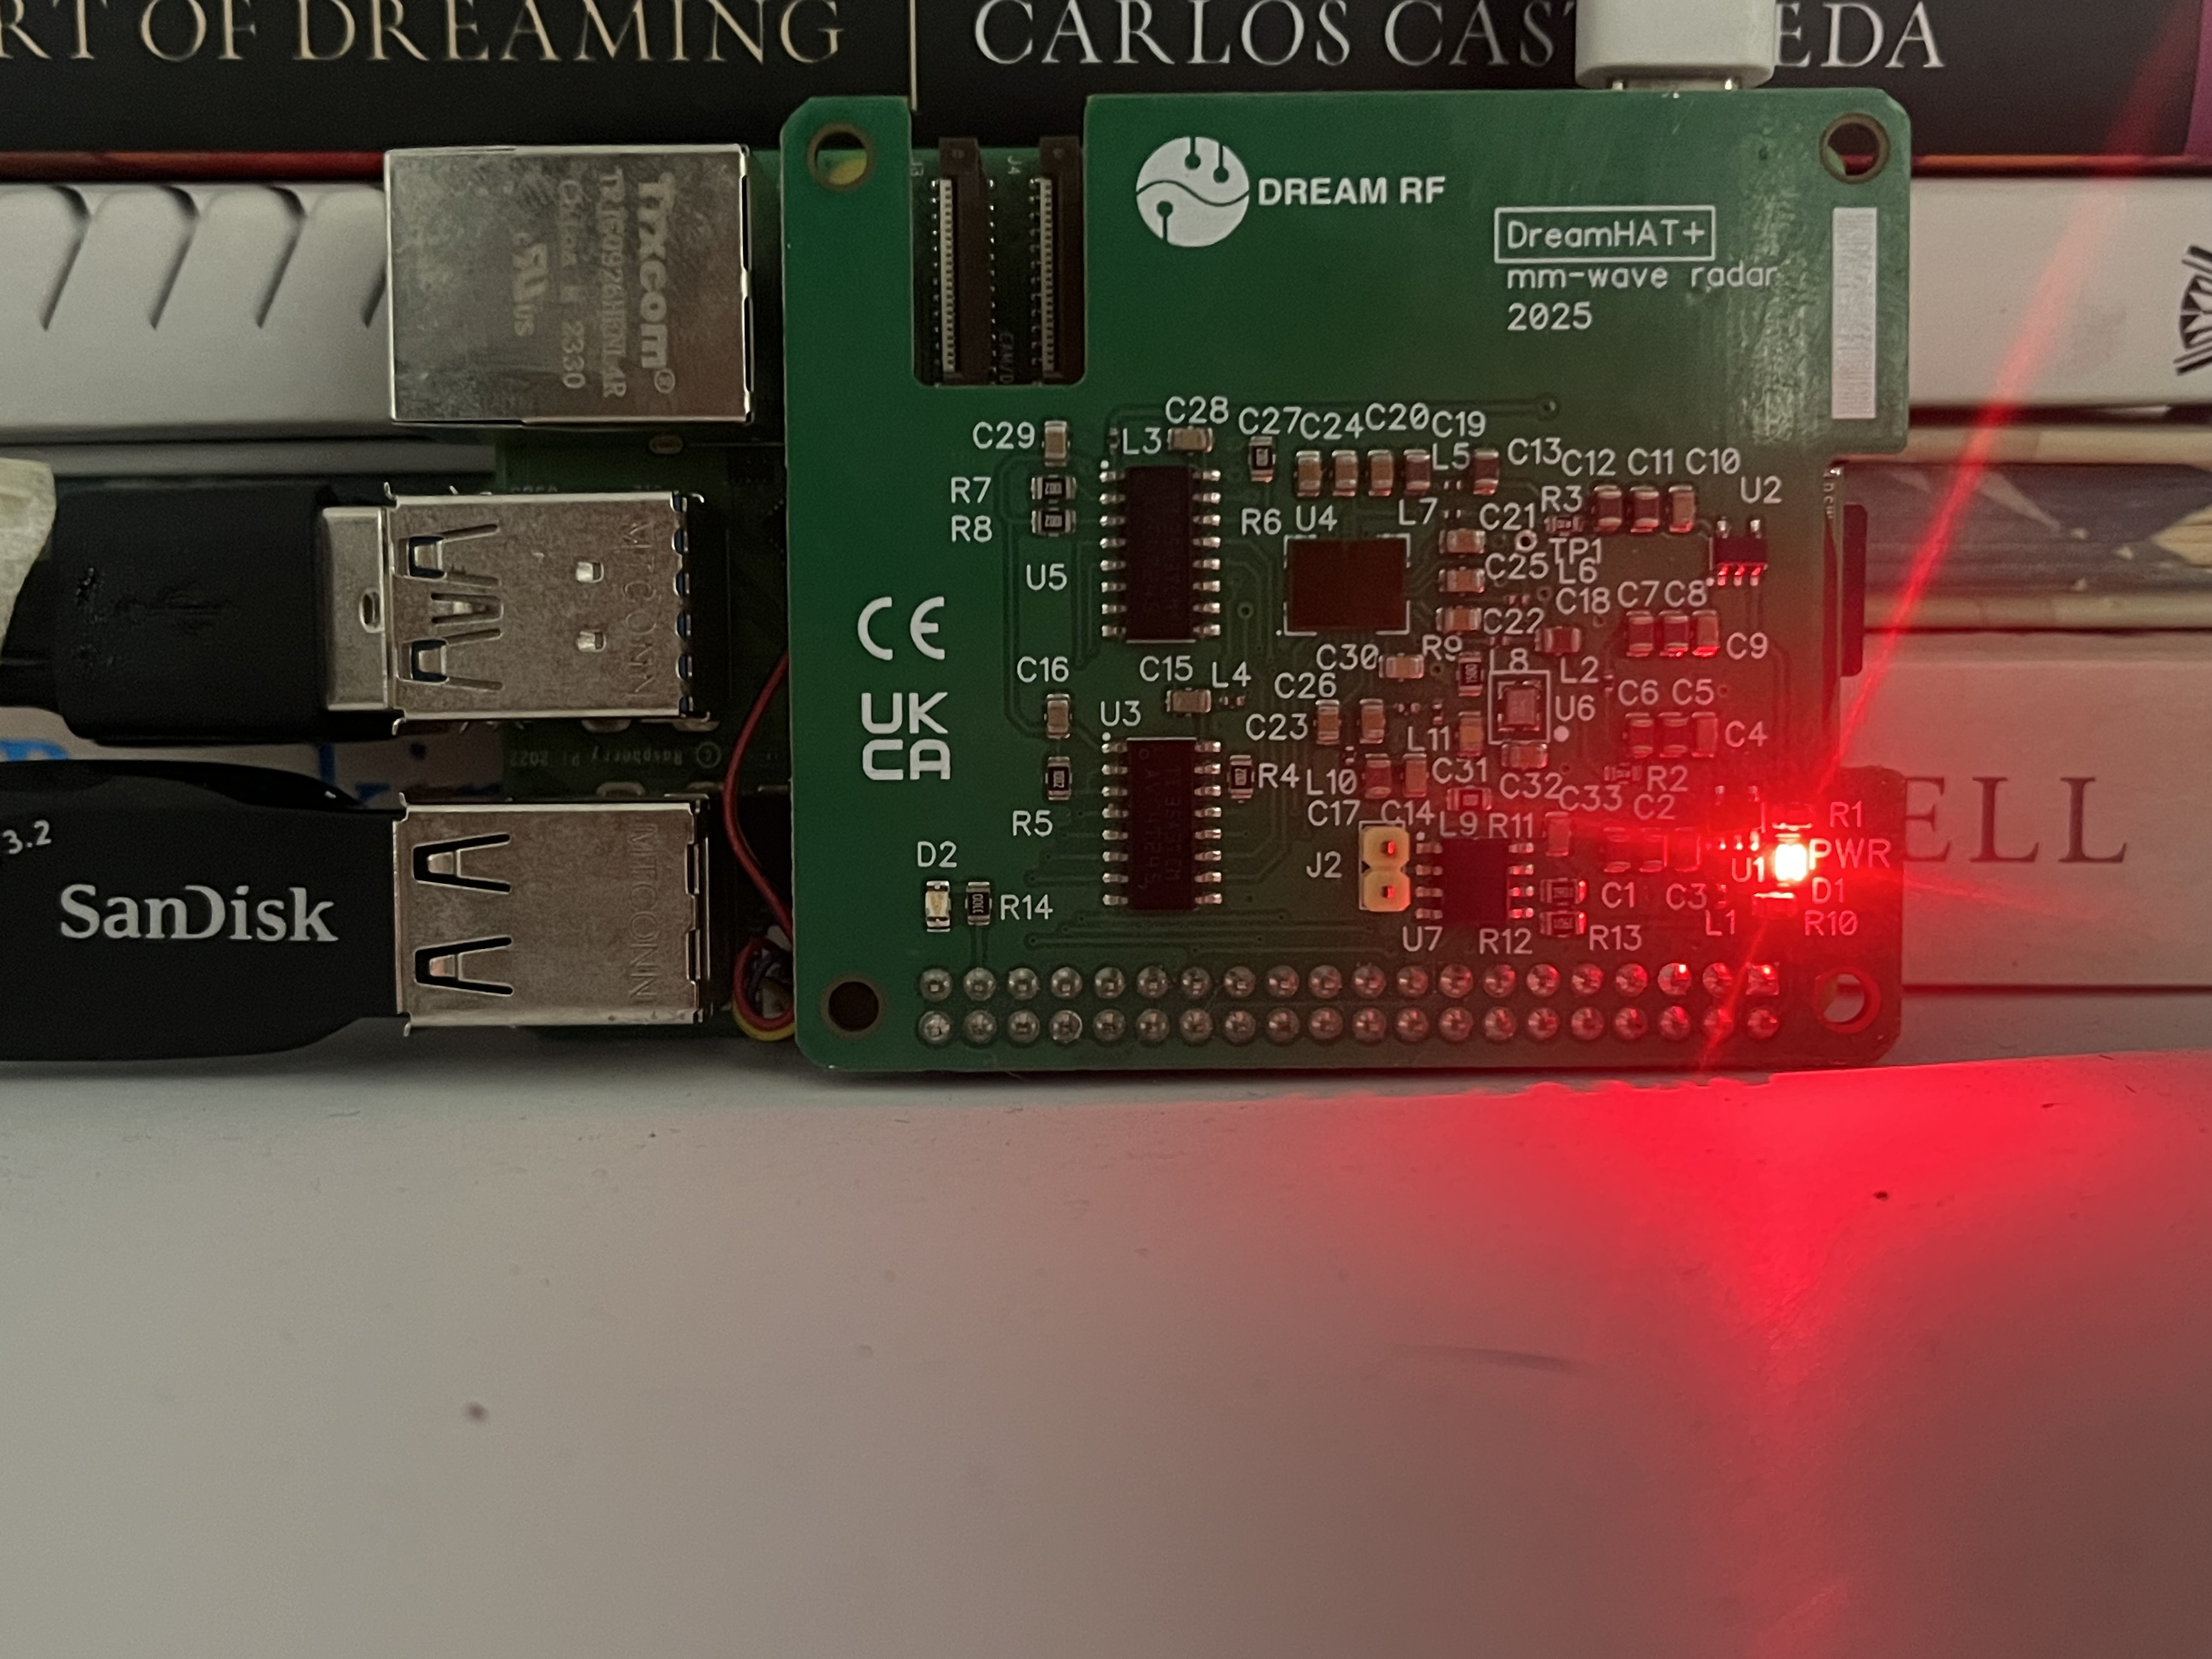
\includegraphics[width=\linewidth,height=2.2cm,keepaspectratio]{IMG_1361.jpeg}\\
{\scriptsize radar: DreamHAT+ on Raspberry Pi}
\end{minipage}\hfill
\begin{minipage}[c]{.49\columnwidth}\centering
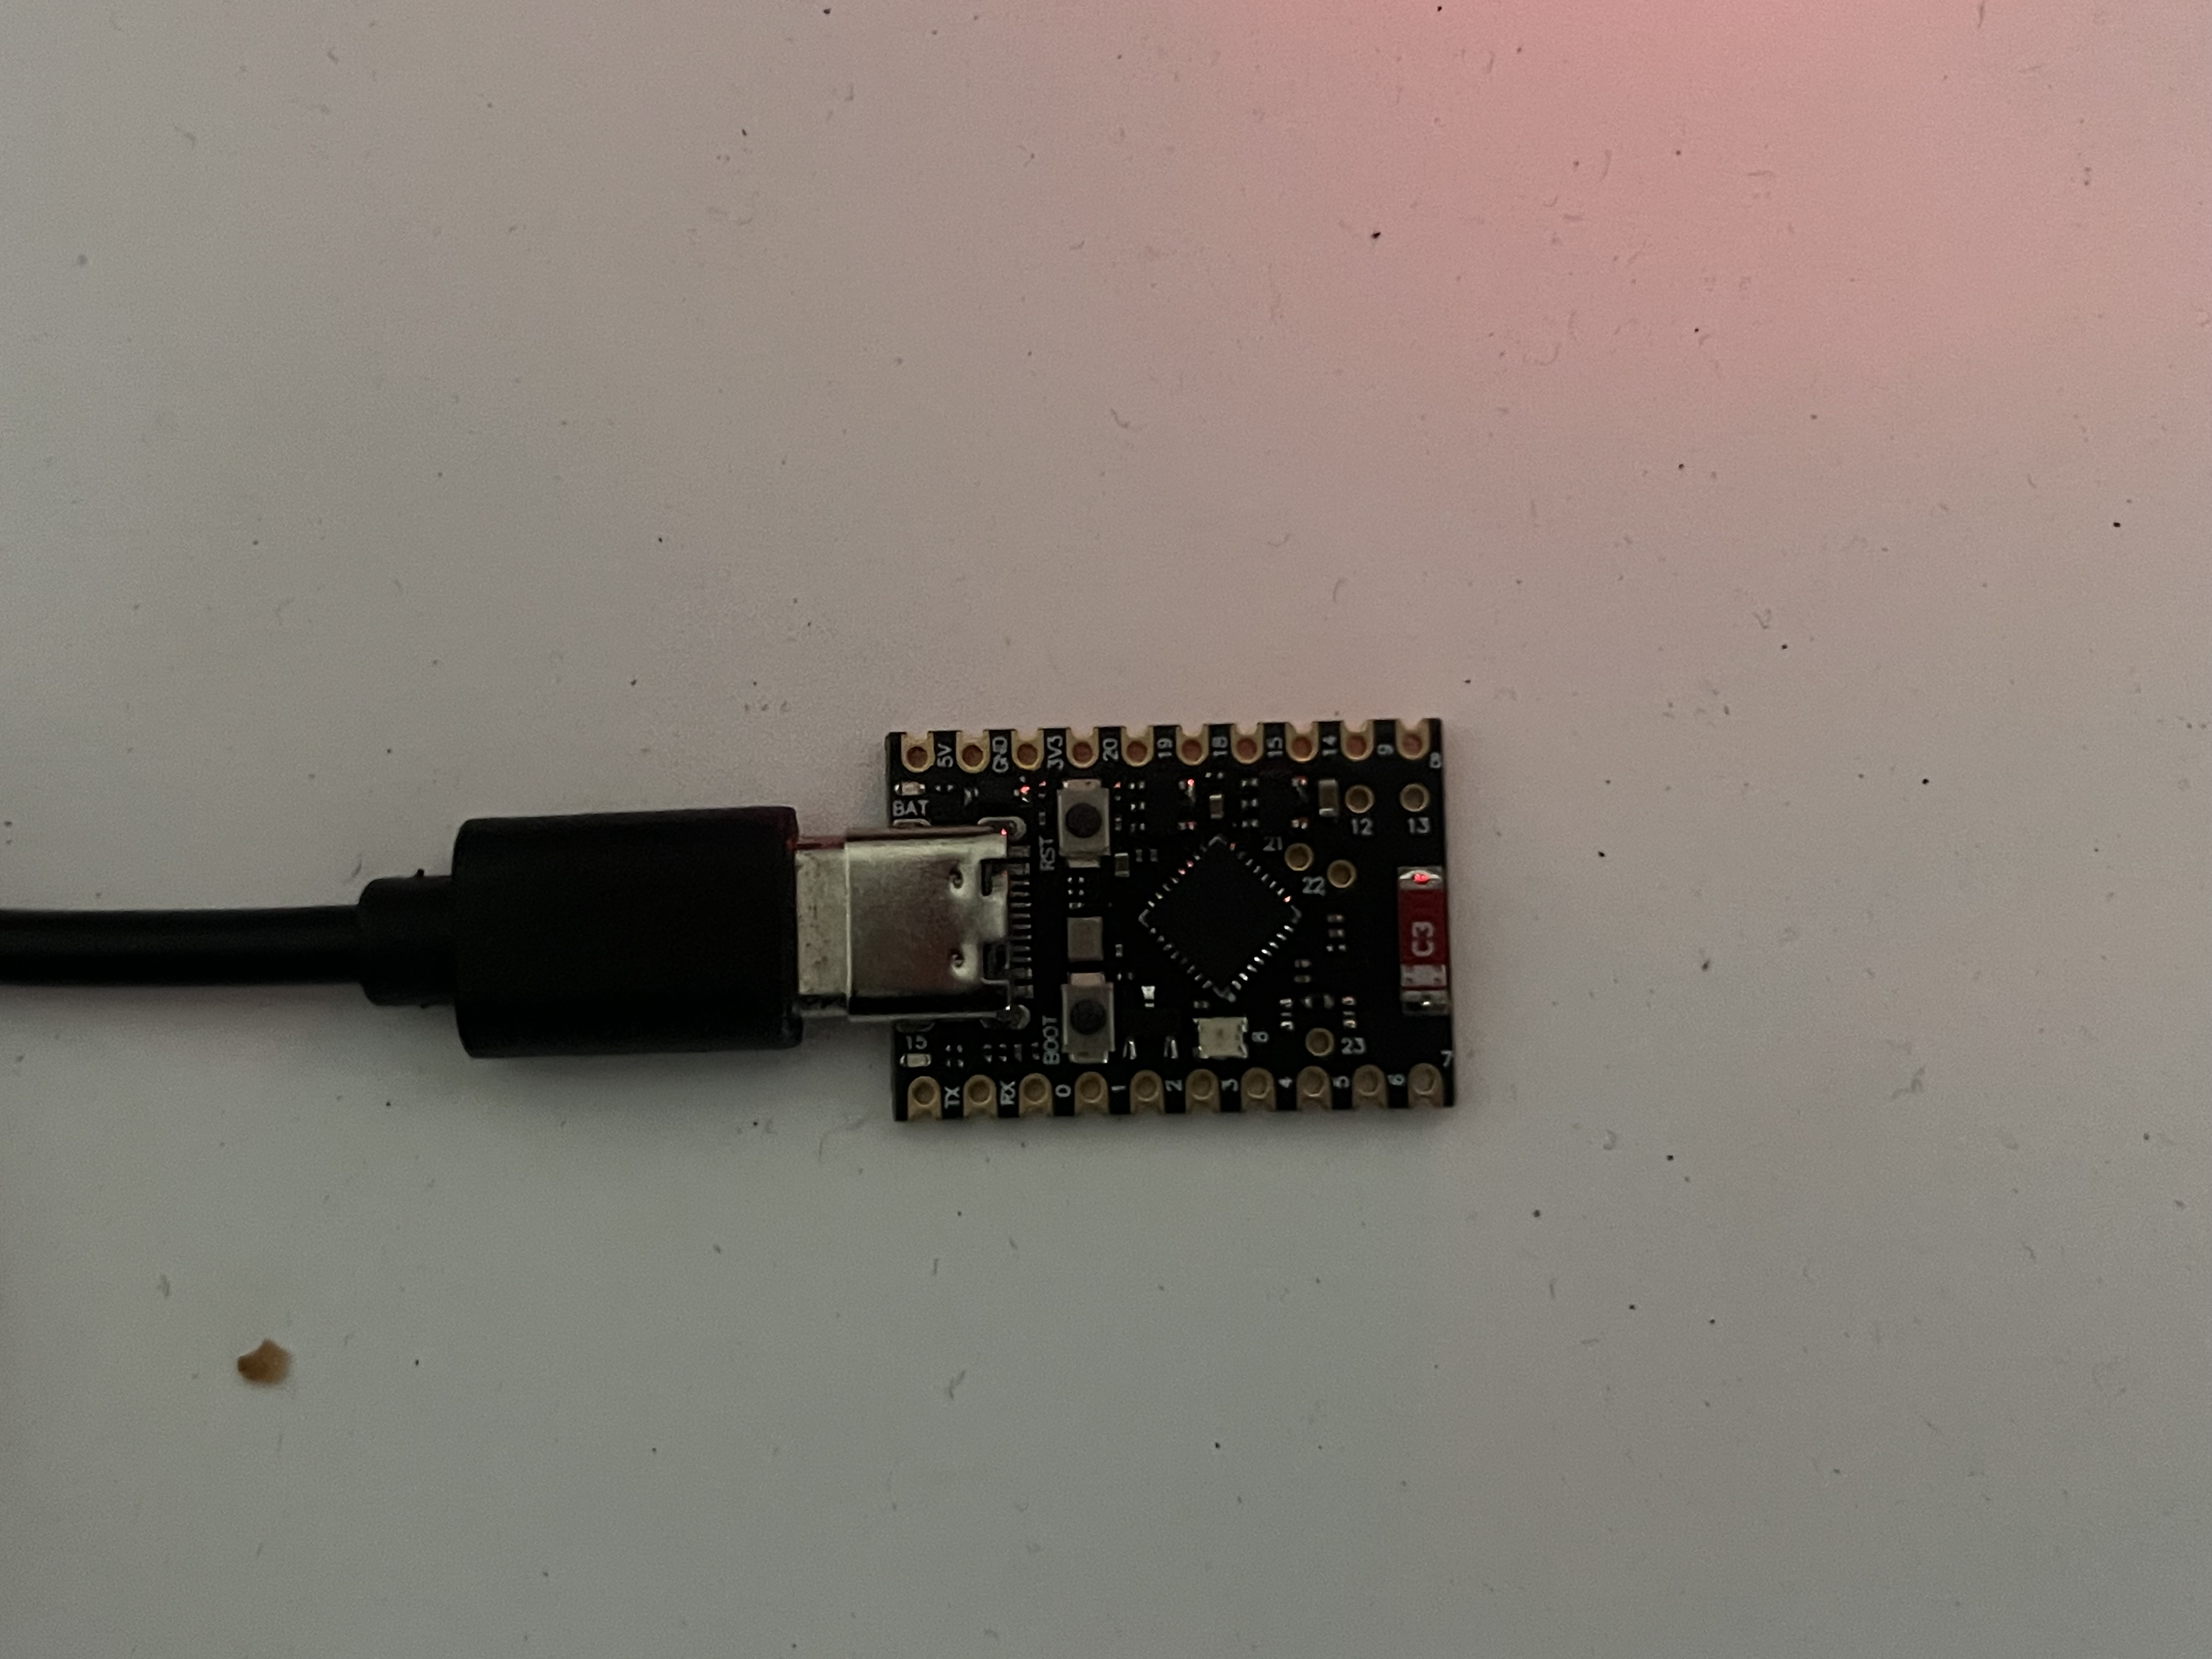
\includegraphics[width=\linewidth,height=2.2cm,keepaspectratio]{IMG_1362.jpeg}\\
{\scriptsize ESP32 board used for CSI}
\end{minipage}
\caption{Room layout, sensor placements, and collection hardware. The co-located FMCW radar and CSI receiver were mounted on wall~4 and wall~2 for training sessions and on wall~3 for validation and test sessions; the CSI sender remained fixed on wall~1. Photographs show the DreamHAT+ mm-wave radar HAT mounted on its Raspberry Pi host (left) and the ESP32 board used for CSI collection (right).}
\label{fig:layout}
\end{figure}

\begin{table}[!b]
\centering\footnotesize
\setlength{\tabcolsep}{3.5pt}
\caption{Sensor configuration. Radar operating band from the BGT60TR13C product brief~\cite{bgt60}; frame structure follows HOOD~\cite{hood}; WiFi settings follow~\cite{wifi}.}
\label{tab:radar}
\begin{tabular}{lcc}\toprule
Configuration & Symbol & Value\\\midrule
\multicolumn{3}{l}{\itshape FMCW radar (BGT60TR13C)}\\
Transmit / receive antennas & $N_{Tx}/N_{Rx}$ & 1 / 3\\
Chirps per frame / samples per chirp & $N_c/N_s$ & 64 / 128\\
Frame period / chirp interval & $T_f/T_{cc}$ & 50\,ms / 391.55\,$\mu$s\\
Start / stop frequency & $f_{\min}/f_{\max}$ & 58 / 63.5\,GHz\\
Bandwidth & $B$ & 5.5\,GHz\\\midrule
\multicolumn{3}{l}{\itshape WiFi CSI (ESP32 sender $\to$ receiver)}\\
Transmit / receive antennas & $N'_{Tx}/N'_{Rx}$ & 1 / 1\\
Channel bandwidth & $B_{\rm wifi}$ & 20\,MHz\\
Reported / retained subcarriers & $K/K'$ & 64 / 52\\
Processed sample grid & $f_s$ & 100\,Hz\\\bottomrule
\end{tabular}
\end{table}

\section{Related Work}\label{sec:related}
\subsection{WiFi CSI sensing}
CSI exposes per-subcarrier channel gains and has been used for presence, activity, and gesture recognition with commodity hardware. DeMan~\cite{deman} detects both moving and stationary humans by combining motion-induced CSI variation with respiration-induced periodicity, and reports that stationary presence is harder because the signal change is small. SHARP~\cite{sharp} targets environment- and person-independent activity recognition by estimating Doppler traces from CSI phase after sanitization, so that the learned representation depends less on static multipath. LiteHAR~\cite{litehar} replaces deep networks with random convolution kernels and a linear classifier, achieving competitive accuracy with a fraction of the training cost. Our earlier work~\cite{wifi} processes amplitude from ESP32 access points for activity recognition in smart homes and motivates the amplitude-only CSI features used here. These studies generally evaluate on the same device placement used for training or on held-out subjects; placement shift remains a known weakness, and our CSI-only result quantifies it for a fixed-threshold classifier.

\subsection{FMCW radar presence detection}
Millimeter-wave FMCW radar supplies range and Doppler information that does not depend on a separate transmitter link. HOOD~\cite{hood} trains a reconstruction-based detector on the Infineon BGT60TR13C and treats presence detection as an out-of-distribution problem, using range--Doppler inputs and a 60.1--61.1\,GHz ramp in its reported configuration. We use the same radar family but work from logged RD, RA, RE, and XY maps and compute low-dimensional descriptors (energy, temporal variability, peak-to-background) rather than training a reconstruction network, which keeps the models small enough to be summarized in a language-model prompt.

\subsection{Radar--WiFi fusion and explanation}
Chen \emph{et al.}~\cite{fusion} fuse radar and WiFi for cross-scene activity recognition and report that fusion is more stable than either modality alone when the scene changes. We examine the same claim for a binary occupancy task with both early feature concatenation and late probability averaging. For model interpretation, SHAP~\cite{shap} estimates each descriptor's contribution to a prediction; we use it to report which descriptors the frozen models rely on. Supplying model outputs and signal statistics to a large language model for a decision and a textual rationale is a newer practice, and we evaluate whether such rationales add information beyond the supplied model predictions.

\section{Problem Definition}\label{sec:problem}
For each minute $m$, decide whether the room is empty ($y_m=0$) or occupied ($y_m=1$) from the CSI amplitude stream and the logged radar maps recorded in that minute. A classifier $f$ and cutoff $\tau$ may be fitted only on training placements $\mathcal{P}_{\rm train}$ (walls 2 and 4) and validation data, while evaluation occurs at $p^\ast\notin\mathcal{P}_{\rm train}$ (wall 3), whose descriptor distribution differs from training; no component may be updated with data from $p^\ast$. We compare the CSI, radar, early-fusion, and late-fusion views under this protocol and ask an LLM, given the descriptor statistics and frozen model outputs, to produce a decision and rationale measured against the same labels.

\section{System Model}\label{sec:system}
Let $y_m\in\{0,1\}$ denote empty or occupied in minute $m$. A CSI packet supplies a complex gain $h_i[k]=|h_i[k]|e^{j\phi_i[k]}$ on retained subcarrier $k$; we use the amplitude $|h_i[k]|$. Following HOOD~\cite{hood}, an FMCW chirp is $s(t)=\exp[j2\pi(f_ct+Bt^2/(2T_c))]$ for $0<t<T_c$, with bandwidth $B$ and chirp duration $T_c$; fast-time and chirp-axis FFTs yield range and Doppler. The available radar stream contains logged RD, RA, RE, and XY maps, from which we compute energy, temporal variability, and a peak-to-background proxy rather than HOOD's reconstruction score. The classifier returns $p_m=P(y_m=1\mid x_{1,m},x_{2,m})$. Early fusion concatenates CSI and radar descriptors before classification; late fusion averages separately fitted CSI and radar probabilities. Figure~\ref{fig:layout} shows the room and sensor placements and Table~\ref{tab:radar} lists the sensor configuration. The BGT60TR13C operates in the 58--63.5\,GHz band~\cite{bgt60}; HOOD's reported ramp of 60.1--61.1\,GHz~\cite{hood} lies inside this band. The exact ramp used in each capture is not stored in the available manifests, so Table~\ref{tab:radar} reports the device band.

\section{Data Collection and Processing}\label{sec:data}
\subsection{Collection protocol}
All data were collected from one subject in the single room shown in Fig.~\ref{fig:layout}. The FMCW radar and the CSI receiver are co-located on one mount; the CSI sender is fixed on wall~1. Training sessions were recorded with the mount on wall~2 and on wall~4. Validation and test sessions were recorded with the mount on wall~3, a placement absent from training, to simulate an unseen domain. Each session runs the multimodal collection (CSI and radar logged together) for a fixed duration under one condition: the subject is present in the room and the session is labeled \emph{occupied}, or the subject leaves and the session is labeled \emph{empty}. Labels are therefore assigned per session, not per frame, and no session contains an occupancy transition.

\subsection{Data sets and preprocessing}
Figure~\ref{fig:sizes} summarizes the data sets. The development collection provides 273 recorded training minutes (187 empty, 86 occupied) and 192 recorded validation minutes (112 empty, 80 occupied). Because occupied is the minority class in both development sets, we synthesize occupied minutes by perturbing each set's own recorded occupied minutes at the descriptor level: Gaussian noise, gain drift, mixup between occupied minutes, and temporal resampling, in rotation. This adds 101 synthetic training and 32 synthetic validation minutes, giving balanced sets of 374 and 224 minutes (1,496 and 896 fifteen-second windows). Four multilink test captures (two per class) provide 1,440 fifteen-second windows and 360 minute buckets (180 per class) and are never augmented. Each capture has one label, so minutes are nested within captures. Multilink CSI averages two links per window, unlike single-link development data. An occupied-only calibration session recorded at the training placements is excluded because it cannot inform a two-class rule. Windows without usable CSI are retained as radar-only windows; their CSI descriptors receive training medians. Sleep is occupied where present.

\begin{figure}[!t]
\centering
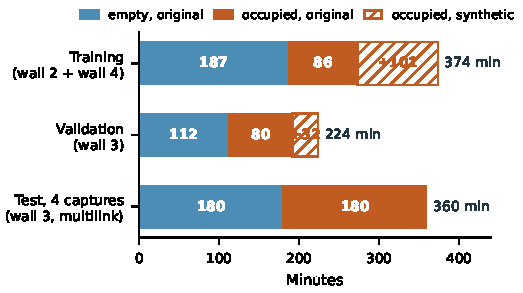
\includegraphics[width=.85\columnwidth]{data_sizes.pdf}
\caption{Data sizes in minutes per class: recorded (solid) and synthesized occupied minutes added for class balance (hatched). Test captures are never augmented.}
\label{fig:sizes}
\end{figure}

\subsection{Physical and hierarchical PCA descriptors}
Candidates include CSI amplitude/variance, RD/RA/RE/XY map summaries, and an SNR proxy: $10\log_{10}$ of nonmasked RD peak over median RD power. A development-only screen retains descriptors with consistent training/validation AUC direction and minimum direction-adjusted AUC .55. Figure~\ref{fig:stable} shows the retained RA and RE temporal-variability descriptors, whose direction persists on multilink test. Three peak measures reverse on test; RA and RE means fail the development screen. Each modality also carries a three-level hierarchical PCA. Level 1 projects one-second CSI dots (mean/std of the 52 subcarrier amplitudes) and radar dots (flattened mean RD map) onto a two-component basis fitted on training seconds. Level 2 stacks five consecutive level-1 coordinate pairs (10 values) and fits a two-component PCA on training five-second blocks; level 3 stacks three consecutive level-2 pairs (6 values) and fits a two-component PCA on training fifteen-second windows. Every level is thus fitted on the training output of the level below, and validation and test seconds are only projected. Blocks with fewer than two valid seconds and windows with fewer than two valid blocks yield missing values that receive training medians (23\% of training, 4\% of validation, and 14\% of test hierarchical values, reflecting sparse joint CSI/radar validity in the training captures). The level-2 bases explain .50/.29 (CSI) and .49/.35 (radar) of block variance and the level-3 bases .48/.20 and .49/.37. Each fifteen-second window summarises the hierarchy by the mean and standard deviation of its level-1 and level-2 PC1/PC2 coordinates and its level-3 PC1/PC2 coordinates (ten values per modality). Model inputs below always combine the physical descriptors with these hierarchical PCA descriptors; Fig.~\ref{fig:pca} shows the three levels for test data.

\begin{figure}[!t]
\centering
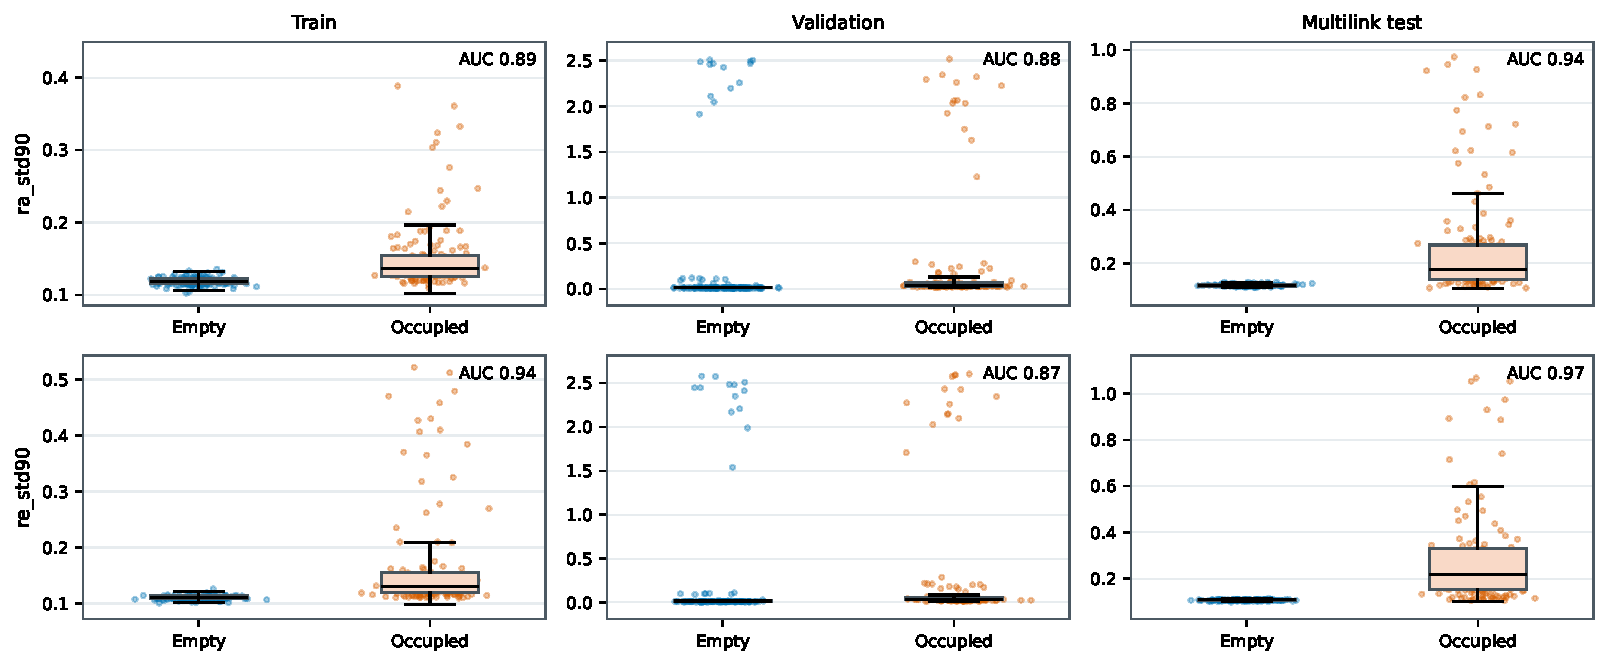
\includegraphics[width=.92\columnwidth]{stable_descriptor_box_scatter.pdf}
\caption{RA and RE variability by class in the training, validation, and multilink test sets.}
\label{fig:stable}
\end{figure}

\begin{figure}[!t]
\centering
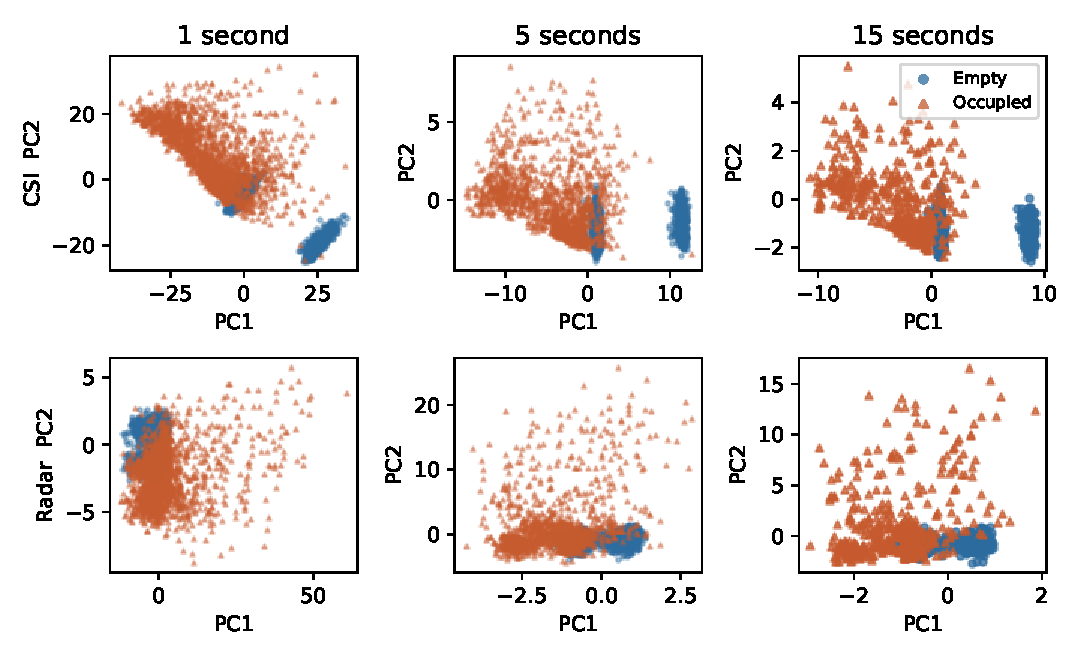
\includegraphics[width=\columnwidth,height=3.3cm]{hierarchical_pca.pdf}
\caption{Hierarchical PCA coordinates (PC1 vs PC2) at the one-second, five-second, and fifteen-second levels for CSI (top) and radar (bottom); multilink test points projected through training-fitted bases, no test fitting.}
\label{fig:pca}
\end{figure}

\section{Predictive Models and Evaluation}\label{sec:models}
We fit RF, GBM, SVM, and a two-hidden-layer MLP (64/32 units) on CSI, radar, and their early descriptor concatenation, each with five random seeds. Late fusion averages same-family CSI and radar probabilities with fixed equal weights. The balanced training set fits missing-value medians, scalers, and model weights; the balanced validation set fixes each seed's cutoff by balanced accuracy, and mean validation-minute AUC over the five seeds selects each view's model and the conventional (ML) and neural (DL) reference models. All choices precede multilink evaluation. Minute probabilities average four fifteen-second outputs; window comparisons use the same minute-fitted cutoff. Test data update no model component.

Classifier vectors contain 18 CSI inputs (eight physical descriptors, each averaged over the window's three five-second rows: amplitude mean/std/90th percentile; rolling-variance mean/90th percentile/maximum; temporal variance; Doppler fraction; and ten hierarchical PCA descriptors: mean/std of the one-second and five-second PC1/PC2 and the fifteen-second PC1/PC2) and 32 radar inputs (22 physical descriptors: SNR mean/maximum; mean, 90th percentile, variability, frame delta, and peak for each RD, RA, RE, and XY map; and ten hierarchical PCA descriptors), giving 50 early-fusion inputs. Each view has training-fitted medians and $z$ scores. Validation fixes the CSI RF (ML reference) and early-fusion MLP (DL reference) cutoffs at .635 and .250; Fig.~\ref{fig:workflow} shows their frozen path.

\begin{figure}[H]
\centering
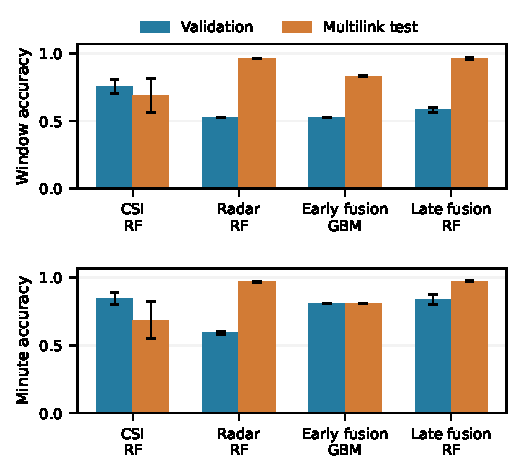
\includegraphics[width=.78\columnwidth]{frozen_comparison.pdf}
\caption{Window and minute accuracy on validation (blue) and multilink test (orange), using validation-fixed models and thresholds.}
\label{fig:pass}
\end{figure}

\section{Language-Model Inference}\label{sec:llm}
Each LLM receives 29 minute means: CSI amplitude mean/std and rolling variance; radar SNR, RA/RE/XY variability 90th percentiles, RA/RE frame deltas; and the twenty hierarchical PCA descriptors of both modalities. One request combines a system rule with a JSON user body that adds training-class mean/std, two labeled training-minute examples per class, and each reference's validation-fixed cutoff, balanced accuracy, minute probability, and decision (Fig.~\ref{fig:workflow}). The system rule asks the LLM to respect model agreement and compare cutoff margins with descriptor statistics on disagreement. IDs are shuffled; capture names, labels, and test-batch ranks are excluded. Output probabilities use a fixed .5 decision cutoff. Three runs cover all 224 validation and 360 test minutes with the same frozen prompt.

\begin{figure*}[!t]
\centering
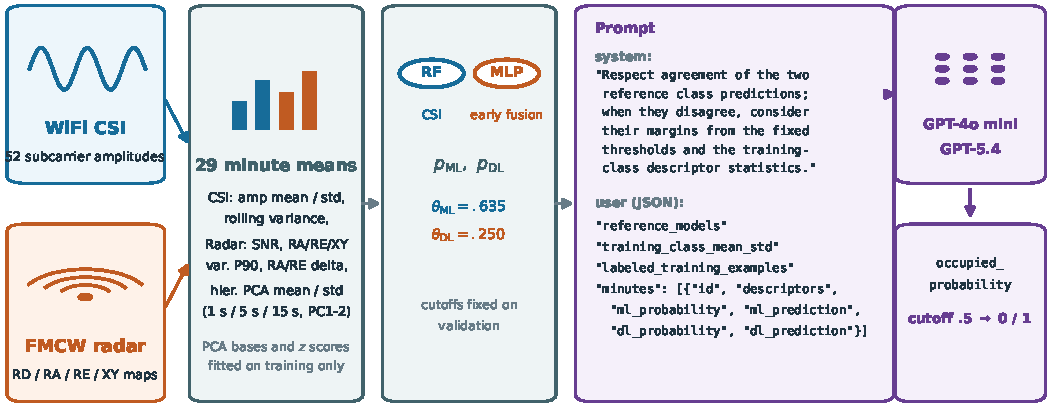
\includegraphics[width=.66\textwidth]{frozen_pipeline.pdf}
\caption{Frozen descriptor-to-LLM path. Twenty-nine minute-mean descriptors and the CSI RF and early-fusion MLP reference probabilities with their validation-fixed cutoffs enter a single chat request; the card shows the system rule and the JSON user keys. The LLM returns an occupancy probability thresholded at .5.}
\label{fig:workflow}
\end{figure*}

\begin{table*}[!t]
\centering\scriptsize\setlength{\tabcolsep}{2pt}\renewcommand{\arraystretch}{1.0}
\caption{Six multilink minutes (three per class). $A/V$: CSI amplitude/rolling-variance mean; $S$: radar SNR; $R_A/R_E/X$: radar variability. References are CSI RF / early-fusion MLP; LLM reasons are verbatim.}
\label{tab:explain}
\begin{tabular}{@{}lp{.19\textwidth}p{.055\textwidth}p{.325\textwidth}p{.325\textwidth}@{}}
\toprule
ID/actual & Signal summary & Ref. $p$ & GPT-4o mini: prediction, reason & GPT-5.4: prediction, reason \\
\midrule
% Generated by E2/export_explainability_rows_v3.py; reasons are verbatim.
m0133/E & CSI $A/V$: 33.22/0.010\newline Radar $S$: 7.58\newline $R_A/R_E/X$: 0.12/0.11/0.11 & 0.65/\newline 0.00 & \textbf{O (0.65)}. High CSI amplitude and PC1 mean; ML output supports occupancy. & \textbf{E (0.20)}. CSI amplitude/SNR and motion stats look empty-like; radar PCs also near empty. ML barely occupied 0.6485, but DL strongly empty 0.0001. \\
\addlinespace[2pt]
m0286/E & CSI $A/V$: 32.82/0.011\newline Radar $S$: 7.46\newline $R_A/R_E/X$: 0.12/0.11/0.11 & 0.64/\newline 0.00 & \textbf{O (0.64)}. High CSI amplitude and PC1 mean; ML output indicates occupancy. & \textbf{E (0.19)}. CSI motion and SNR are empty-like despite shifted PCA basis; radar PCs remain near empty. ML barely occupied 0.6353, DL strongly empty 0.0002. \\
\addlinespace[2pt]
m0215/E & CSI $A/V$: 23.47/0.008\newline Radar $S$: 7.71\newline $R_A/R_E/X$: 0.12/0.11/0.11 & 0.62/\newline 0.03 & \textbf{E (0.62)}. Low CSI amplitude and PC1 mean; ML output suggests emptiness. & \textbf{E (0.08)}. CSI amplitude, SNR, ra/re spread and deltas match empty; radar PCs modest and non-occupied. Both models predict empty: ML 0.6179, DL 0.0259. \\
\addlinespace[2pt]
m0146/O & CSI $A/V$: 16.27/0.037\newline Radar $S$: 15.49\newline $R_A/R_E/X$: 0.48/0.58/0.36 & 0.70/\newline 1.00 & \textbf{O (0.70)}. High SNR and significant radar PC1 mean; ML output confirms occupancy. & \textbf{O (0.99)}. CSI high SNR, ra/re spreads, deltas, extreme PCs indicate occupancy; radar PC1/PC2 strongly match occupied examples. Both models occupied: ML 0.696, DL 1.0. \\
\addlinespace[2pt]
m0209/O & CSI $A/V$: 16.65/0.018\newline Radar $S$: 7.57\newline $R_A/R_E/X$: 0.16/0.17/0.14 & 0.81/\newline 1.00 & \textbf{O (0.81)}. Strong radar evidence and high ML probability indicate occupancy. & \textbf{O (0.87)}. CSI very low amplitude and strongly shifted PCs support occupancy; radar motion stats are weaker, only mildly occupied-like. Both models occupied: ML 0.8136, DL 1.0. \\
\addlinespace[2pt]
m0147/O & CSI $A/V$: 19.30/0.008\newline Radar $S$: 7.79\newline $R_A/R_E/X$: 0.17/0.23/0.15 & 0.79/\newline 1.00 & \textbf{O (0.79)}. Radar PC1 mean suggests occupancy; ML output supports this. & \textbf{O (0.72)}. CSI lower amplitude, elevated re/xy spread, shifted PCs suggest occupancy; radar PCs conflict, looking atypical/empty-leaning. Both models still occupied: ML 0.7944, DL 0.9979. \\
\bottomrule

\end{tabular}
\end{table*}

\section{Results and Discussion}\label{sec:results}
\begin{table}[!t]
\centering\footnotesize\setlength{\tabcolsep}{3.5pt}
\caption{Fifteen-second models on physical + hierarchical PCA descriptors, minute evaluation, validation-fixed thresholds; mean $\pm$ sd over five seeds (sd omitted when $<.005$). $^\ast$~view leader by mean validation-minute AUC.}
\label{tab:primary}
\begin{tabular}{llllll}
\toprule
View & Model & Val. AUC & Val. acc. & Test acc. & Test AUC\\
\midrule
\multirow{4}{*}{CSI} & RF$^\ast$ & .88$\pm$.04 & .85$\pm$.05 & .69$\pm$.14 & .82$\pm$.03 \\
 & GBM & .68 & .69 & .83 & .85 \\
 & SVM & .14 & .53 & .48 & .37 \\
 & MLP & .45$\pm$.13 & .56$\pm$.05 & .60$\pm$.09 & .72$\pm$.07 \\
\midrule
\multirow{4}{*}{Radar} & RF$^\ast$ & .57$\pm$.02 & .59$\pm$.01 & .97$\pm$.00 & 1.00$\pm$.00 \\
 & GBM & .55 & .59 & .81 & .97 \\
 & SVM & .47$\pm$.00 & .51 & .92$\pm$.00 & 1.00 \\
 & MLP & .56$\pm$.07 & .69$\pm$.04 & .77$\pm$.15 & .97$\pm$.02 \\
\midrule
\multirow{4}{*}{Early fusion} & RF & .61$\pm$.11 & .63$\pm$.06 & .97$\pm$.00 & .99$\pm$.00 \\
 & GBM$^\ast$ & .83 & .81 & .81 & .96 \\
 & SVM & .44$\pm$.00 & .50 & .80$\pm$.00 & .92 \\
 & MLP & .58$\pm$.18 & .64$\pm$.12 & .72$\pm$.16 & .95$\pm$.03 \\
\midrule
\multirow{4}{*}{Late fusion} & RF$^\ast$ & .87$\pm$.04 & .84$\pm$.04 & .97$\pm$.00 & 1.00$\pm$.00 \\
 & GBM & .71 & .73 & .81 & .94 \\
 & SVM & .16 & .53 & .96 & 1.00 \\
 & MLP & .56$\pm$.06 & .68$\pm$.04 & .59$\pm$.09 & .93$\pm$.04 \\
\bottomrule
\end{tabular}
\end{table}

\begin{figure}[!t]
\centering
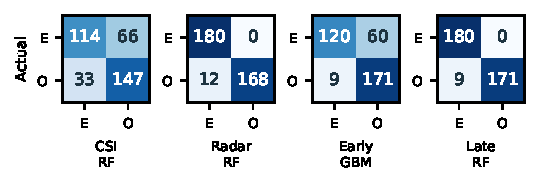
\includegraphics[width=.85\columnwidth]{primary_cm.pdf}
\caption{Test confusion matrices for Table~\ref{tab:primary}'s view leaders over 360 minutes. E/O: empty/occupied; rows are actual, columns predicted.}
\label{fig:primarycm}
\end{figure}

\subsection{CSI-only results}
Validation selects the CSI RF (AUC .88, accuracy .85, the highest validation AUC of all sixteen candidates), but it falls to $.69\pm.14$ test minute accuracy (window .69), misclassifying 66 empty and 33 occupied minutes for seed~0 (Table~\ref{tab:primary}, Fig.~\ref{fig:primarycm}). The CSI GBM transfers better (.83 test) with lower validation AUC (.68). CSI separates the development placements well, but its descriptor distribution shifts on multilink; because it ranks first on validation, the CSI RF becomes the ML reference.

\subsection{Radar-only results}
Validation ranks the radar view weakly (RF AUC .58, accuracy .59), yet the selected RF reaches .969 test minute accuracy (window .962, AUC 1.00), missing 12 occupied minutes and no empty one. The radar GBM (.81) and SVM (.92) score lower on test. The test evaluates two captures per class whose labels do not change within a capture.

\subsection{Sensor fusion: early features}
Early fusion concatenates the 50 inputs. The GBM leader (validation AUC .83, accuracy .81) reaches .808 test minute accuracy (window .833), predicting occupied for 60 of 180 empty minutes; the RF scores $.97\pm.00$ on test but only .61 validation AUC. The early-fusion MLP (test $.72\pm.16$) is the DL reference because no MLP view scores higher on validation.

\subsection{Decision fusion: late probabilities}
Late fusion averages same-family CSI and radar probabilities with weight $1/2$ fixed before evaluation. The RF pair reaches .837 validation and $.975\pm.003$ test minute accuracy (window .961, test AUC 1.00), misclassifying 9 occupied minutes; the SVM pair follows at .961 test. Late fusion is again the strongest selectable view and the only one that combines a high validation AUC (.87) with transfer to the test placement.

\subsection{Descriptor importance}
Table~\ref{tab:shap} reports interventional Shapley estimates for the ML reference (CSI RF), the DL reference (early-fusion MLP), and the late-fusion GBM. Each of 24 random descriptor orders starts from a random training window; 24 validation windows (12 per class) are explained. The CSI RF relies on CSI amplitude P90 (.157), std (.074), and mean (.049), followed by total variation (.026) and the five-second and one-second PC1 means (.024 each). The DL reference concentrates on RA energy mean (.432) and P90 (.413), CSI amplitude mean (.208), and RE energy mean (.176). The late-fusion GBM uses CSI amplitude P90 (.219), RE variability (.132), CSI amplitude mean (.095), and RE frame delta (.081); its largest hierarchical term is the one-second CSI PC1 mean (.032). Hierarchical PCA descriptors therefore enter mainly through the CSI PC1 means at the one- and five-second levels. These values describe model reliance, not causal sensor importance~\cite{shap}; neither SHAP sampling nor model choice uses multilink labels.

\begin{table}[!t]
\centering\scriptsize\setlength{\tabcolsep}{2pt}
\caption{Mean absolute interventional Shapley contribution to occupied probability for the ML reference (CSI RF), the DL reference (early-fusion MLP), and the late-fusion GBM (Late); 24 validation windows, training-window background.}
\label{tab:shap}
\begin{tabular}{@{}llllllll@{}}
\toprule
Descriptor & ML & DL & Late & Descriptor & ML & DL & Late\\
\midrule
CSI amplitude mean & .049 & .208 & .095 & RA energy mean & -- & .432 & .001 \\
CSI amplitude std & .074 & .007 & .020 & RA energy P90 & -- & .413 & .000 \\
CSI amplitude P90 & .157 & .126 & .219 & RA variability P90 & -- & .023 & .001 \\
CSI rolling-var. mean & .011 & .004 & .004 & RA frame delta & -- & .091 & .000 \\
CSI rolling-var. P90 & .007 & .004 & .004 & RA peak/background & -- & .088 & .006 \\
CSI rolling-var. max & .003 & .006 & .005 & RE energy mean & -- & .176 & .000 \\
CSI total variation & .026 & .007 & .014 & RE energy P90 & -- & .128 & .003 \\
CSI Doppler fraction & .013 & .005 & .008 & RE variability P90 & -- & .032 & .132 \\
CSI 1 s PC1 mean & .024 & .095 & .032 & RE frame delta & -- & .071 & .081 \\
CSI 1 s PC2 mean & .005 & .081 & .014 & RE peak/background & -- & .128 & .000 \\
CSI 1 s PC1 std & .015 & .007 & .008 & XY energy mean & -- & .042 & .000 \\
CSI 1 s PC2 std & .009 & .015 & .003 & XY energy P90 & -- & .045 & .000 \\
CSI 5 s PC1 mean & .024 & .026 & .006 & XY variability P90 & -- & .080 & .011 \\
CSI 5 s PC2 mean & .006 & .003 & .007 & XY frame delta & -- & .096 & .000 \\
CSI 5 s PC1 std & .015 & .005 & .011 & XY peak/background & -- & .034 & .002 \\
CSI 5 s PC2 std & .015 & .011 & .002 & Radar 1 s PC1 mean & -- & .004 & .000 \\
CSI 15 s PC1 & .011 & .080 & .013 & Radar 1 s PC2 mean & -- & .048 & .000 \\
CSI 15 s PC2 & .007 & .009 & .004 & Radar 1 s PC1 std & -- & .003 & .000 \\
Radar SNR mean & -- & .003 & .000 & Radar 1 s PC2 std & -- & .006 & .000 \\
Radar SNR max & -- & .002 & .000 & Radar 5 s PC1 mean & -- & .032 & .000 \\
RD energy mean & -- & .002 & .000 & Radar 5 s PC2 mean & -- & .009 & .000 \\
RD energy P90 & -- & .009 & .000 & Radar 5 s PC1 std & -- & .035 & .000 \\
RD variability P90 & -- & .002 & .000 & Radar 5 s PC2 std & -- & .002 & .000 \\
RD frame delta & -- & .011 & .000 & Radar 15 s PC1 & -- & .030 & .000 \\
RD peak/background & -- & .047 & .001 & Radar 15 s PC2 & -- & .013 & .000 \\
\bottomrule
\end{tabular}
\end{table}

\subsection{Language-model evaluation}
GPT-4o mini scores $58.6\pm2.3$\% on validation and $61.1\pm2.2$\% on multilink test; GPT-5.4 scores $80.4\pm1.5$\% and $94.4\pm0.2$\%, respectively (mean $\pm$ sample standard deviation over three runs). GPT-4o mini did not pass the prespecified .80 test gate for the second model; GPT-5.4 was run regardless and the waiver is recorded. For run~1 on all 360 test minutes, the confusion counts (true empty, false occupied, false empty, true occupied) are $(51,129,2,178)$ for GPT-4o mini, $(177,3,17,163)$ for GPT-5.4, $(114,66,33,147)$ for the CSI RF reference, and $(152,28,10,170)$ for the early-fusion MLP reference. GPT-4o mini predicts occupied for most minutes, following the CSI RF reference whose cutoff (.635) sits just below many empty-minute probabilities; GPT-5.4 weighs the DL reference and the physical descriptors and reaches .944, below the late-fusion RF's .975 but above both references. Run-to-run spread reuses the same minutes, so it is not an independent-sample interval.

\subsection{LLM explanation check}
For a separate qualitative check, we selected three empty and three occupied test minutes by fixed-seed sampling within the four captures, without considering model outcomes. Both LLMs received the same 29 descriptors and frozen reference outputs as above, with a request for a short reason; this prompt differs and is excluded from the accuracy estimate. Table~\ref{tab:explain} reports their complete concise replies. GPT-4o mini follows the ML reference and calls two of the three empty minutes occupied, citing CSI amplitude and PC1 means. GPT-5.4 resolves all six correctly, noting that the ML probability is only marginally above its cutoff while the DL reference and the physical descriptors indicate empty. These are model-generated rationales, not causal explanations of raw signals.

\section{Limitations}\label{sec:limits}
Labels are constant within each capture, so adjacent minutes are correlated, occupancy transitions are not measured, and capture replication is two per class. The unseen domain is a placement change for one subject in one room, the per-capture radar ramp is not logged (Table~\ref{tab:radar} reports the device band), and descriptor-level synthetic minutes add no information beyond the recorded ones. The LLM prompt asks for agreement with two supplied decisions, and a plausible rationale is not an independent explanation of the measurement.

\section{Conclusion}\label{sec:conclusion}
Physical descriptors and mean/std summaries of a three-level hierarchical training-fitted PCA drive the fifteen-second models, and descriptor-level augmentation balances the training and validation sets. Under validation-fixed models and thresholds, the selected views reach .687 CSI, .969 radar, .808 early-fusion, and .975 late-fusion minute accuracy on the unseen test placement; the CSI RF that ranks first on validation does not transfer, while late probability fusion does. GPT-4o mini reaches .611 test accuracy by following the CSI reference; GPT-5.4 reaches .944. Neither exceeds the late-fusion RF, and generated rationales can echo a weak reference. The remaining gaps are within-session occupancy transitions, additional subjects and rooms, and logged per-capture radar settings.

\bibliographystyle{IEEEtran}
\bibliography{refs}
\end{document}

